% Method schematic (version 2): one flow, top to bottom, ALL positions relative.
% Compile standalone from the manuscript folder:  pdflatex method_schematic2.tex
% (loads ../figure/fig3.png for the municipality map)
%
% HOW TO MOVE THINGS
%  * every plot is a named node `parea` (size \pw x \ph cm); curves are drawn in the
%    plot's own local coordinates (0..\pw, 0..\ph), so they follow the node.
%  * to move a plot: edit its `at ([shift={(dx,dy)}]othernode)` / `below=..of` line.
%  * to resize all plots: change \pw / \ph (curves rescale automatically).
\documentclass[tikz,border=6pt]{standalone}
\usepackage{amsmath}
\usepackage{graphicx}
\usetikzlibrary{arrows.meta,calc,positioning,fit,backgrounds,shapes.misc}

\usepackage[scaled]{helvet}
\renewcommand{\familydefault}{\sfdefault}

\definecolor{tNavy}{HTML}{1A3B5D}
\definecolor{tTeal}{HTML}{1B9E77}
\definecolor{tOrng}{HTML}{E6550D}
\definecolor{pFill}{HTML}{FBFCFE}
\definecolor{pEdge}{HTML}{C7D2E0}
\definecolor{cA15}{HTML}{F2A65A}   % light orange
\definecolor{cA50}{HTML}{9E2B25}   % dark red
\definecolor{cFd}{HTML}{15497A}    % fertility : dark blue
\definecolor{cFl}{HTML}{7FB3E0}    % fertility : light blue

% ------------------------------------------------------------------ parameters
\def\pw{3}     % plot width  (cm)
\def\ph{1.5}   % plot height (cm)

% plot decoration: axes + title + x label + y label, attached to node #1.
% optional first argument = how far left the y label sits (default 2pt)
\newcommand{\pdeco}[5][2pt]{%
  \draw[ax] (#2.south west)--(#2.south east);
  \draw[ax] (#2.south west)--(#2.north west);
  \node[ttl,anchor=south] (#2-t) at ([yshift=3pt]#2.north) {#3};
  \node[sub,anchor=north] (#2-x) at ([yshift=-1pt]#2.south) {#4};
  \node[sub,rotate=90,anchor=south] (#2-y) at ([xshift=-#1]#2.west) {#5};
}

\begin{document}
\begin{tikzpicture}[
  font=\sffamily,
  >={Stealth[length=5pt]},
  panel/.style={draw=pEdge,fill=pFill,rounded corners=4pt,line width=.9pt},
  box/.style={draw=pEdge,fill=white,rounded corners=3pt,line width=.7pt},
  parea/.style={minimum width=\pw cm,minimum height=\ph cm,inner sep=0pt,outer sep=0pt},
  ttl/.style={font=\scriptsize\bfseries,text=tNavy},
  sub/.style={font=\tiny,text=black!60},
  ax/.style={black!45,line width=.5pt},
  zero/.style={black!50,line width=.5pt,densely dashed},
  a50/.style={draw=cA50,line width=1pt},
  fdk/.style={draw=cFd,line width=1pt},
  flt/.style={draw=cFl,line width=1pt},
  agg/.style={draw=cA15!50!cA50,line width=1pt},   % mix of the two age colours
  flow/.style={->,draw=black!55,line width=1pt},
]

% ====================================================================
% 1. National births (top, centred)
% ====================================================================
\node[parea] (nb) at (0,0) {};
\pdeco{nb}{National births}{Time}{Births}
\begin{scope}[shift={(nb.south west)}]
  \draw[a50] plot[domain=0.05:\pw-0.05,samples=100,smooth]
    (\x,{0.55+0.17*\x+0.14*sin(3*\x/\pw*360)});
\end{scope}

% ====================================================================
% 2. Population (slightly below, to the left of National births)
% ====================================================================
\node[parea] (pop) at ([shift={(-5.2,-0.9)}]nb) {};
\pdeco{pop}{Population}{Time}{Pop. size}
\begin{scope}[shift={(pop.south west)}]
  \draw[a50] (0.05,0.35) .. controls (1,0.5) and (2,0.8) .. (\pw-0.05,1.1);
\end{scope}

% ====================================================================
% 3. Big box with three plots: Trend | Season | Shift in childbearing age
% ====================================================================
\node[parea,below=2.9cm of nb] (se) {};              % middle (centred under nb)
\node[parea,left =1.6cm of se] (tr) {};
\node[parea,right=1.6cm of se] (sh) {};

\pdeco{tr}{Trend}{Time}{Birth rate}
\pdeco{se}{Season}{Time}{Birth rate}
\pdeco{sh}{Shift in childbearing age}{Age}{Fertility}

% trend: straight decreasing line
\begin{scope}[shift={(tr.south west)}]
  \draw[a50] (0.05,1.2)--(\pw-0.05,0.35);
\end{scope}
% season: seasonal sine (3 seasons), no trend
\begin{scope}[shift={(se.south west)}]
  \draw[a50] plot[domain=0.05:\pw-0.05,samples=100,smooth]
    (\x,{0.75+0.3*sin(3*\x/\pw*360)});
\end{scope}
% shift in childbearing age: same fertility curve, shifted horizontally
\begin{scope}[shift={(sh.south west)}]
  \draw[fdk] plot[domain=0.05:\pw-0.05,samples=80,smooth]
    (\x,{0.1+1.1*exp(-((\x-1.15)/0.42)*((\x-1.15)/0.42))});
  \draw[flt] plot[domain=0.05:\pw-0.05,samples=80,smooth]
    (\x,{0.1+1.1*exp(-((\x-1.75)/0.42)*((\x-1.75)/0.42))});
\end{scope}

% the big box wraps the three plots and their labels
\begin{scope}[on background layer]
  \node[panel,fill=white,fit=(tr-y)(tr-t)(tr-x)(se-t)(se-x)(sh-t)(sh-x)(sh),inner sep=7pt] (bigbox) {};
\end{scope}

% national births -> each of the three plots
\draw[flow] (nb-x.south) -- (tr-t.north);
\draw[flow] (nb-x.south) -- (se-t.north);
\draw[flow] (nb-x.south) -- (sh-t.north);

% ====================================================================
% 4. National expectation (below the big box, a bit to the right) + text box
% ====================================================================
\node[parea,below=1.9cm of bigbox,xshift=2.2cm] (ne) {};
\pdeco{ne}{National expectation}{Time}{Births}
\begin{scope}[shift={(ne.south west)}]
  % expected line only
  \draw[agg,dashed] plot[domain=0.05:\pw-0.05,samples=100,smooth]
    (\x,{0.6125+0.0583*\x+0.11*sin(3*\x/\pw*360)});
\end{scope}

\node[box,text width=4.2cm,align=center,font=\scriptsize,inner sep=5pt,left=1.1cm of ne] (cf)
  {Counterfactual birth with stable birth rate and accounting for shift in childbearing age and population changes.};

% trend and shift -> expectation ; season -> expectation (faded, crossed out)
\draw[flow] (tr-x.south) -- ([xshift=-0.9cm]ne-t.north);
\draw[flow] (sh-x.south) -- ([xshift= 0.9cm]ne-t.north);
\draw[flow,opacity=.4] (se-x.south) -- (ne-t.north);
\node[cross out,draw=red,line width=1.8pt,minimum size=0.3cm,inner sep=0pt]
  at ($(se-x.south)!0.5!(ne-t.north)$) {};

% ====================================================================
% 5. National excess/deficit (below, a bit right)  and  Municipality-level map (below, a bit left)
% ====================================================================
\node[parea] (nex) at ([shift={(2.8,-3.8)}]ne) {};
\pdeco[9pt]{nex}{National excess/deficit of births}{Time}{Excess/deficit}
\begin{scope}[shift={(nex.south west)}]
  \def\obsx{0.7875-0.0583*\x+0.14*sin(3*\x/\pw*360)}      % observed
  \def\expx{0.6125+0.0583*\x+0.11*sin(3*\x/\pw*360)}      % expected
  \draw[zero] (0,{\ph/2})--(\pw,{\ph/2});
  \node[sub,anchor=east] at (0,{\ph/2}) {0};
  % excess/deficit = observed - expected (x2.5 for visibility)
  \draw[agg] plot[domain=0.05:\pw-0.05,samples=100,smooth]
    (\x,{\ph/2+2.5*((\obsx)-(\expx))});
\end{scope}

% municipality-level map (figure 3), no axes
\node[inner sep=0pt] (mun) at ([shift={(-2.9,-4.2)}]ne)
  {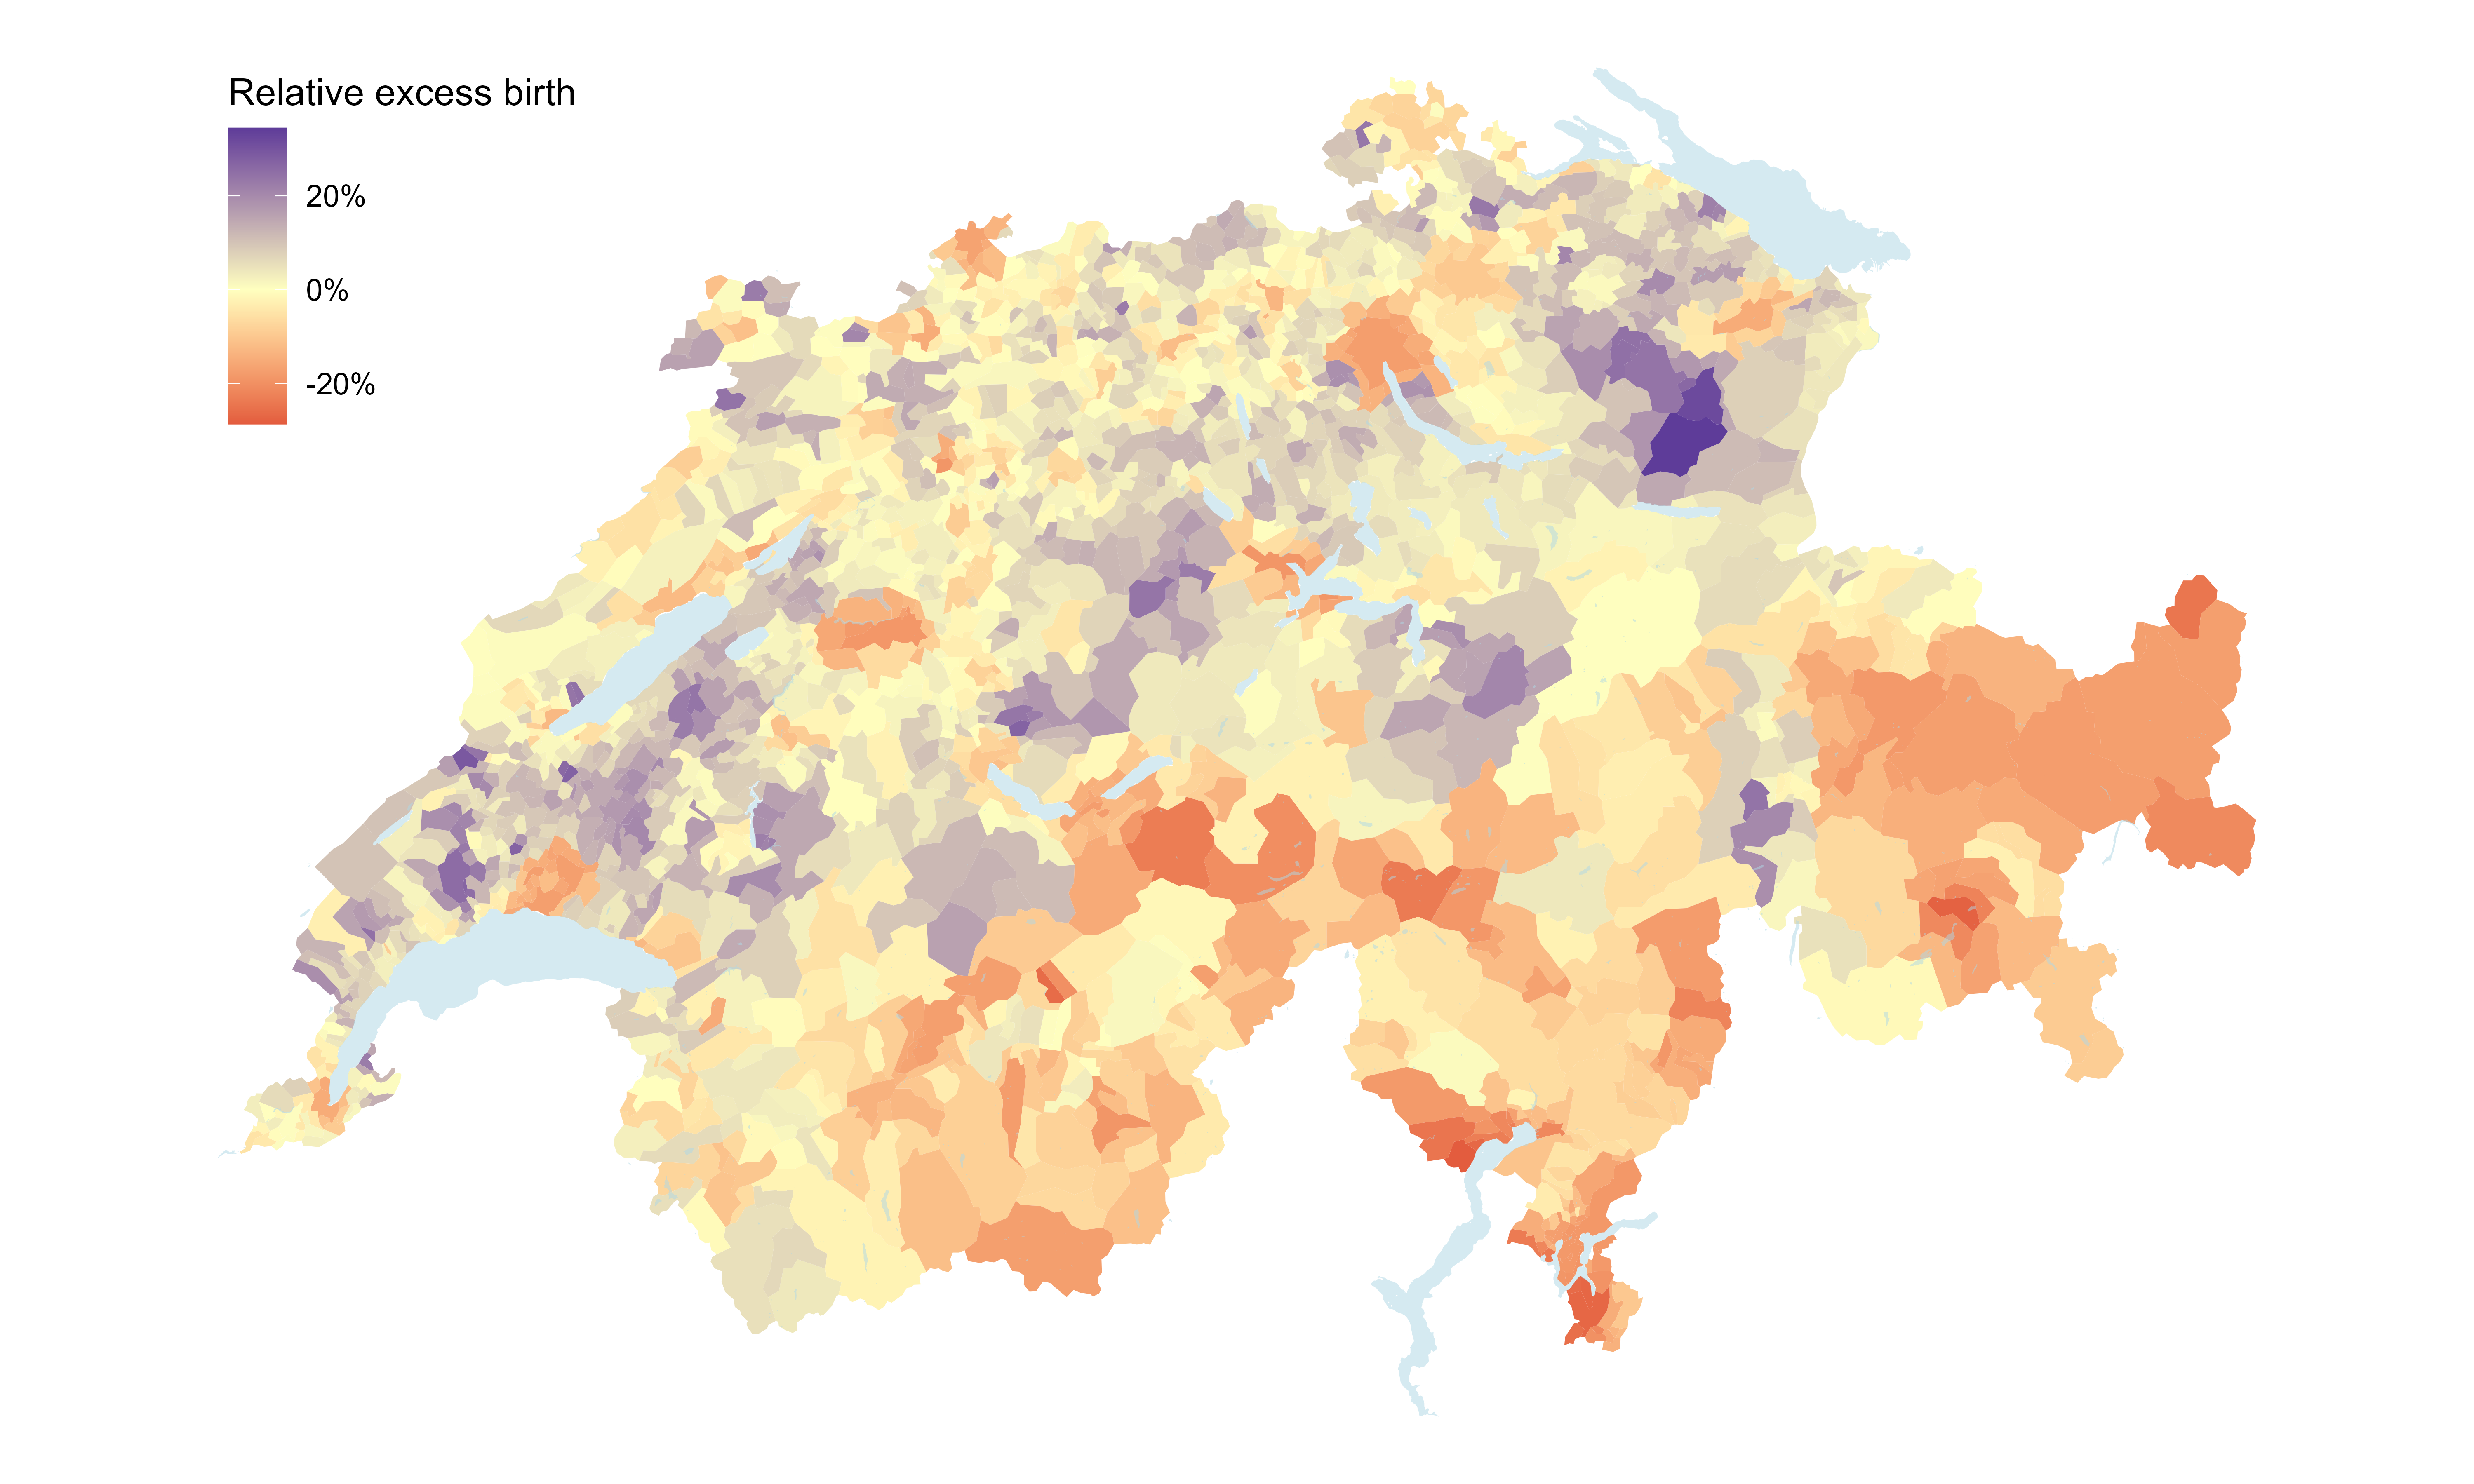
\includegraphics[width=4.8cm]{../figure/fig3.png}};
\node[ttl,anchor=south] (mun-t) at ([yshift=3pt]mun.north) {Municipality-level};

% national expectation -> national / municipality-level
\draw[flow] (ne-x.south) -- (nex-t.north);
\draw[flow] (ne-x.south) -- (mun-t.north);

% ====================================================================
% 6. Municipal excess/deficit (below the municipality map), two coloured lines
% ====================================================================
\node[parea,below=1.9cm of mun] (mex) {};
\pdeco[9pt]{mex}{Municipal excess/deficit of births}{Time}{Excess/deficit}
\begin{scope}[shift={(mex.south west)}]
  \draw[zero] (0,{\ph/2})--(\pw,{\ph/2});
  \node[sub,anchor=east] at (0,{\ph/2}) {0};
  \draw[draw=tTeal,line width=1pt] plot[domain=0.05:\pw-0.05,samples=100,smooth]
    (\x,{\ph/2+0.4-0.27*\x+0.07*sin(3*\x/\pw*360)});
  \draw[draw=tOrng,line width=1pt] plot[domain=0.05:\pw-0.05,samples=100,smooth]
    (\x,{\ph/2-0.25+0.12*\x+0.07*sin(3*\x/\pw*360+60)});
\end{scope}

% ====================================================================
% overall box (single panel). Delete this block for no frame.
% ====================================================================
\begin{scope}[on background layer]
  \node[panel,fit=(pop-y)(pop-t)(nb-t)(bigbox)(cf)(ne-y)(nex-t)(nex-x)(nex-y)(mun)(mun-t)(mex-t)(mex-x)(mex-y),inner sep=12pt] {};
\end{scope}

\end{tikzpicture}
\end{document}
